% Sections 3 and 4: regularization and conclusion.
% Include in main.tex with % Sections 3 and 4: regularization and conclusion.
% Include in main.tex with % Sections 3 and 4: regularization and conclusion.
% Include in main.tex with % Sections 3 and 4: regularization and conclusion.
% Include in main.tex with \input{sec_lambda} before \end{document}.
% Needs fig_rk_lambda.png (made by Code/uonn/uo_nn_lambda_analysis.m).

\section{Effect of regularization}\label{sec:lambdapos}

We now compare the runs with $\lambda\in\{0,\,0.01,\,0.5\}$. As in Section~\ref{sec:lambda0}, the iterations, losses, times and accuracies come from the batch, and the other quantities from \texttt{uo\_nn\_\allowbreak lambda\_\allowbreak analysis.m} (Section~1, Experimental setup). Since the number of GM and BFGS iterations depends on the state of the random generator used by the line search, we also give the mean over the batch run and the five repetitions with other states when we compare iteration counts.

\subsection{Global convergence}\label{sec:lambdaglobal}

\textbf{Theory.} For $\lambda>0$ the objective has a property that it lacks for $\lambda=0$: since the data term is non-negative, $\tilde L(w)\ge\frac{\lambda}{2}\|w\|^2$, so $\tilde L(w)\to\infty$ when $\|w\|\to\infty$. GM and BFGS with a Wolfe line search decrease $\tilde L$ at every iteration, so all iterates stay in the level set $\{w:\tilde L(w)\le\tilde L(w^1)=0.25\}$, which gives
\[
  \|w^k\|\le\sqrt{0.5/\lambda}\;=\;7.1 \text{ for } \lambda=0.01,\qquad 1.0 \text{ for } \lambda=0.5 .
\]
The iterates are therefore bounded and the minimum of $\tilde L$ is attained. For $\lambda=0$ there is no such bound. The loss can keep decreasing while $\|w\|$ grows, because the sigmoid only approaches 0 and 1 for arguments of growing size. In addition, $\lambda I$ is added to the Hessian, $\nabla^2\tilde L=\nabla^2 L+\lambda I$, which raises its smallest eigenvalue by $\lambda$ and lowers its condition number. Both effects should make convergence easier as $\lambda$ grows.

\textbf{Observations.} Table~\ref{tab:convlambda} summarizes the convergence for the three values of $\lambda$.

\begin{table}[h]
\centering
\small
\setlength{\tabcolsep}{3pt}
\begin{tabular}{l ccc ccc ccc}
\toprule
 & \multicolumn{3}{c}{GM} & \multicolumn{3}{c}{BFGS} & \multicolumn{3}{c}{SGM} \\
\cmidrule(lr){2-4}\cmidrule(lr){5-7}\cmidrule(lr){8-10}
$\lambda$ & 0 & 0.01 & 0.5 & 0 & 0.01 & 0.5 & 0 & 0.01 & 0.5 \\
\midrule
Mean iter.\ / epochs & 57.3 & 29.5 & 9.4 & 31.6 & 24.2 & 8.0 & 18.3 & 11.2 & 11.3 \\
Max iter.\ / epochs & 100 & 70 & 13 & 97 & 31 & 9 & 100 & 16 & 14 \\
Not converged & 2 & 0 & 0 & 0 & 0 & 0 & 1 & 0 & 0 \\
Mean, 6 gen.\ states & 57.6 & 31.5 & 9.2 & 33.2 & 25.6 & 6.8 & -- & -- & -- \\
Mean $t$ [s] & 3.18 & 1.62 & 0.50 & 1.78 & 1.37 & 0.47 & 0.33 & 0.24 & 0.26 \\
$\|w^*\|$ & 3.6--6.4 & 1.8--2.4 & .29--.44 & 4.6--35 & 1.8--2.5 & .29--.44 & 4.7--9.6 & 1.8--2.7 & .33--.58 \\
Max $\|\nabla\tilde L(w^*)\|$ & $2.8{\cdot}10^{-3}$ & $9.9{\cdot}10^{-4}$ & $7.7{\cdot}10^{-4}$ & $9.9{\cdot}10^{-4}$ & $9.9{\cdot}10^{-4}$ & $7.4{\cdot}10^{-4}$ & $2.5{\cdot}10^{-2}$ & 0.22 & 0.62 \\
\bottomrule
\end{tabular}
\caption{Convergence for the three values of $\lambda$, over the ten digits. Iterations for GM and BFGS, epochs for SGM. ``Not converged'' means the iteration limit was reached with $\|\nabla\tilde L\|>10^{-3}$ (GM, BFGS) or the 100-epoch limit was reached (SGM). The ``6 generator states'' row is the mean over the batch run and the five repetitions with \texttt{rng(1)}--\texttt{rng(5)}.}
\label{tab:convlambda}
\end{table}

\begin{itemize}
  \item \textbf{GM} converges on all digits for both $\lambda>0$, while at $\lambda=0$ it reached the 100-iteration limit on digits 3 and 8. The mean number of iterations halves from $\lambda=0$ to $\lambda=0.01$ and drops by a further factor of three at $\lambda=0.5$. In the repetitions with other generator states, GM at $\lambda=0$ reached the limit in 18 of 60 runs (always on digits 3, 8 and 9), and for $\lambda>0$ it never needed more than 78 iterations.
  \item \textbf{BFGS} converged on all digits for every $\lambda$, but the worst case improves strongly: from 97 iterations at $\lambda=0$ to 31 and 9. The quantities in the global convergence conditions behave in the same way. Over all BFGS iterations, $\kappa(H_k)$ reached up to $1.6\cdot10^{6}$ for $\lambda=0$, but only $1.2\cdot10^{2}$ for $\lambda=0.01$ and $3.3$ for $\lambda=0.5$. The smallest $\cos\theta_k$ was $0.005$, $0.25$ and $0.94$. For $\lambda>0$ the direction is therefore well away from orthogonal to the gradient, and the condition of Section~\ref{sec:global} holds with a large margin. The line search found a strong Wolfe step in every BFGS iteration for $\lambda>0$. For GM it did so in every iteration except 6 of the 162 iterations on digits 3, 8 and 9 with $\lambda=0.01$.
  \item \textbf{The solution becomes well defined.} At $\lambda=0$, GM and BFGS stop at different points: $\|w^*\|$ is 6.0 for GM and 35 for BFGS on digit 2, and the two final losses differ on every digit (Table~\ref{tab:acc}). The Hessian at the BFGS solutions has small negative eigenvalues on six digits (down to $-5.6\cdot10^{-4}$), so these points are not strict minimizers. For $\lambda>0$, GM and BFGS give the same $\tilde L^*$ to three digits and $\|w^*\|$ within 0.03 on every digit, and the smallest Hessian eigenvalue is 0.011--0.013 for $\lambda=0.01$ and 0.51 for $\lambda=0.5$, that is, about $\lambda$. The observed $\|w^*\|$ is also well inside the bound $\sqrt{0.5/\lambda}$ above.
  \item \textbf{SGM} stopped early on all 20 runs with $\lambda>0$, after 6 to 16 epochs, so in the sense of Section~\ref{sec:global} it converged on every digit. The returned points are, however, further from stationary as $\lambda$ grows: $\|\nabla\tilde L(w^*)\|$ on the full training set is at most $2.5\cdot10^{-2}$ for $\lambda=0$, between $2.3\cdot10^{-2}$ and $0.22$ for $\lambda=0.01$, and between 0.35 and 0.62 for $\lambda=0.5$. The reason for $\lambda=0.5$ is discussed in Section~\ref{sec:lambdaacc}.
\end{itemize}

In summary, regularization makes the global convergence of GM and BFGS easier, both in theory (bounded level sets, a positive definite Hessian at the solution) and in the experiments (no iteration limit reached, well-conditioned $H_k$). It does not help SGM in the same way, because its run length is set by early stopping and not by the gradient.

\subsection{Local convergence and speed}\label{sec:lambdalocal}

\textbf{Conditioning.} The condition number of the Hessian at the solution, $\kappa(\nabla^2\tilde L(w^*))$, is $1.7\cdot10^{2}$--$3.0\cdot10^{2}$ at the GM solutions for $\lambda=0$, 17--69 for $\lambda=0.01$ and 3.1--4.1 for $\lambda=0.5$. For GM the theory predicts a linear rate that gets worse as $\kappa$ grows. With an exact line search the bound on the reduction of $\tilde L-\tilde L^*$ per iteration is $\left(\frac{\kappa-1}{\kappa+1}\right)^2$, which is 0.98, 0.92 and 0.36 for $\kappa=250$, 50 and 4. Figure~\ref{fig:rklambda} shows the gradient norm for digits 4, 6 and 8.

\begin{figure}[h]
  \centering
  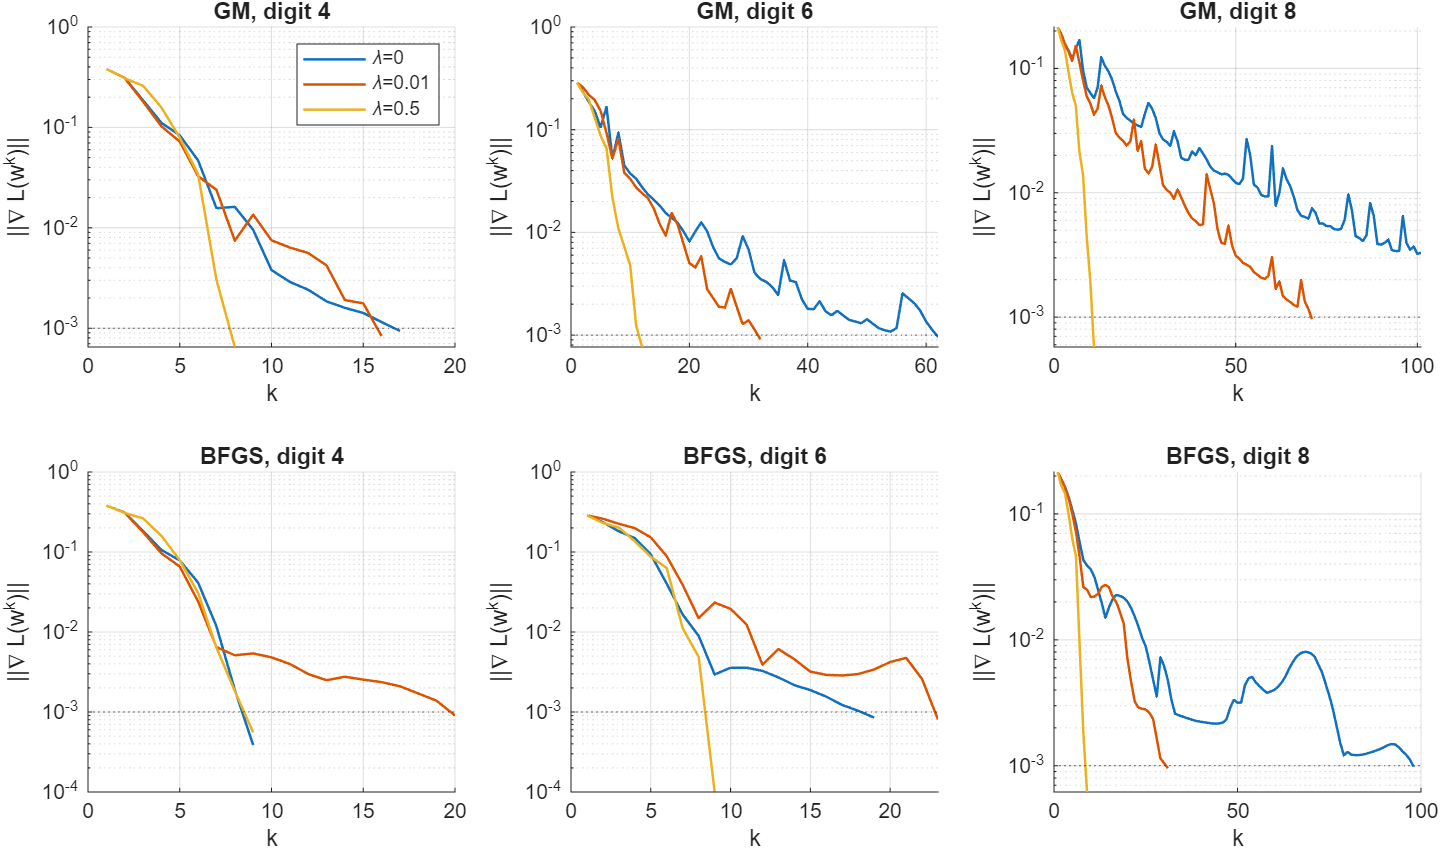
\includegraphics[width=\linewidth]{fig_rk_lambda.png}
  \caption{Gradient norm $\|\nabla\tilde L(w^k)\|$ of GM (top) and BFGS (bottom) on digits 4, 6 and 8, for $\lambda=0$ (blue), $0.01$ (red) and $0.5$ (yellow). The dotted line is the tolerance $10^{-3}$.}
  \label{fig:rklambda}
\end{figure}

\textbf{GM.} The average reduction of the gradient norm per iteration, $(\|\nabla\tilde L(w^{K+1})\|/\|\nabla\tilde L(w^1)\|)^{1/K}$, is on average 0.83 for $\lambda=0$, 0.76 for $\lambda=0.01$ and 0.50 for $\lambda=0.5$ over the ten digits. The ordering is the one predicted by the condition numbers. The observed values are smaller than the bound because the bound is a worst case, and our iterates spend part of the run far from $w^*$. The effect is clearest on digit 8 (Figure~\ref{fig:rklambda}, top right). At $\lambda=0$ the gradient norm still oscillates between $3\cdot10^{-3}$ and $10^{-2}$ after 100 iterations, at $\lambda=0.01$ it decreases more steadily and reaches the tolerance after 70 iterations, and at $\lambda=0.5$ it reaches the tolerance after 10 iterations.

\textbf{BFGS.} For $\lambda=0.5$, BFGS converges in 4 to 12 iterations in all 60 runs, with an average reduction of 0.44 per iteration and a last ratio $r_k$ between 0.02 and 0.34. For $\lambda=0.01$ the average reduction is 0.78, and the median $r_k$ over the last five iterations is 0.87. As for $\lambda=0$ (Section~\ref{sec:local}), we do not see a superlinear phase before the tolerance stops the run.

\textbf{GM against BFGS.} At $\lambda=0$, BFGS needed fewer iterations than GM on all ten digits (mean over the six generator states). At $\lambda=0.5$ this is still the case (6.8 against 9.2 iterations on average). At $\lambda=0.01$, however, BFGS needed fewer iterations only on digits 3, 8, 9 and 0, the four digits with the largest $\kappa(\nabla^2\tilde L(w^*))$ (47 to 69). On the other six digits GM was faster. The largest difference is on digit 7, with 16.2 iterations for GM and 24.7 for BFGS, where $\kappa=21$. On digit 8 the opposite holds, with 69.8 iterations for GM and 29.3 for BFGS. Our explanation is that BFGS mainly helps when the problem is badly conditioned. When $\kappa$ is small, GM is already fast. BFGS starts with $H_1=I$, the same step as GM, and needs several iterations to build a useful approximation of the inverse Hessian. During these iterations its direction deviates from $-\nabla\tilde L$ ($\cos\theta_k$ down to 0.25--0.45 for $\lambda=0.01$) without yet pointing more directly at the minimum. We did not test this explanation, for example with a scaled initial matrix $H_1$.

\textbf{Time.} The time per iteration does not depend on $\lambda$: 0.053 to 0.059\,s per iteration for both GM and BFGS and all three values (total time divided by total iterations). This is expected, since the regularization term only adds $O(n)$ operations to the loss and the gradient. The total time therefore follows the number of iterations, and for GM falls from 3.18\,s to 1.62\,s and 0.50\,s. SGM needs 11 epochs on average for both $\lambda>0$ and takes 0.24 to 0.26\,s, so $\lambda$ has no systematic effect on its run time.

\subsection{Accuracy}\label{sec:lambdaacc}

Table~\ref{tab:acclambda} gives the mean accuracies and the number of test errors, split into false negatives (target images that were rejected) and false positives (other images that were accepted).

\begin{table}[h]
\centering
\small
\setlength{\tabcolsep}{4pt}
\begin{tabular}{l ccc ccc ccc}
\toprule
 & \multicolumn{3}{c}{GM} & \multicolumn{3}{c}{BFGS} & \multicolumn{3}{c}{SGM} \\
\cmidrule(lr){2-4}\cmidrule(lr){5-7}\cmidrule(lr){8-10}
$\lambda$ & 0 & 0.01 & 0.5 & 0 & 0.01 & 0.5 & 0 & 0.01 & 0.5 \\
\midrule
Mean $\tilde L^*$ & 0.0074 & 0.0495 & 0.197 & 0.0065 & 0.0495 & 0.197 & 0.0072 & 0.0589 & 0.295 \\
Mean train acc.\ [\%] & 99.22 & 99.15 & 92.96 & 99.20 & 99.15 & 92.97 & 99.08 & 97.84 & 56.71 \\
Mean test acc.\ [\%] & 99.14 & 99.10 & 87.56 & 98.96 & 99.10 & 87.58 & 99.30 & 99.24 & 91.68 \\
Min test acc.\ [\%] & 96.6 & 96.2 & 64.4 & 96.4 & 96.2 & 64.2 & 97.4 & 98.0 & 89.6 \\
False negatives (of 500) & 5 & 6 & 0 & 6 & 6 & 0 & 8 & 27 & 416 \\
False positives (of 4500) & 38 & 39 & 622 & 46 & 39 & 621 & 27 & 11 & 0 \\
\bottomrule
\end{tabular}
\caption{Accuracy for the three values of $\lambda$, over the ten digits. The test errors are summed over the ten test sets of 500 images, which together contain 500 target and 4500 non-target images. The mean test accuracy of the always-negative classifier is 90.0\%.}
\label{tab:acclambda}
\end{table}

\textbf{$\lambda=0.01$.} The accuracy is practically the same as for $\lambda=0$: the mean test accuracy is 99.10\% for both GM and BFGS, against 99.14\% and 98.96\% without regularization, and the mean training accuracy decreases by less than 0.1 points. On single digits the test accuracy changes by at most 5 images (1 percentage point), and the changes go in both directions. Regularization is meant to reduce overfitting, and at $\lambda=0$ there was little to reduce: the network has only 35 weights for 5000 training samples, and the training and test accuracies were already similar (Section~\ref{sec:acc}). The main effect of $\lambda=0.01$ on accuracy is that GM and BFGS now return the same classifier. At $\lambda=0$ their test accuracies differed by up to 4 images on a digit, at $\lambda=0.01$ they are identical on all ten digits, because both methods find the same minimizer.

SGM behaves differently at $\lambda=0.01$. Its mean training accuracy drops to 97.84\% (93.0\% on digit 8 and 95.3\% on digit 3), while its test accuracy stays at 99.24\%. Its errors move towards false negatives (27 false negatives and 11 false positives, against 8 and 27 at $\lambda=0$). Since SGM selects its weights on the test loss and the test set is 90\% non-target, weights that reject doubtful images are favoured. The test accuracy of SGM should therefore again be read as slightly optimistic.

\textbf{$\lambda=0.5$: GM and BFGS.} Strong regularization makes the classifier clearly worse. The mean test accuracy falls to 87.6\%, which is below the 90.0\% of a classifier that always answers ``not the target''. On digit 8 it is only 64.4\%. All 622 test errors are false positives: no target image is missed, but up to 179 of the 458 non-target images are accepted on digit 8 (true negative rate 61\%). Since the test images are the same for every target, the true digit of each test image is known from the labels of the ten test sets. For target 8, 173 of the 178 false positives are 0s, 3s, 6s and 9s (45, 52, 34 and 42). For target 9 they are 0s, 3s and 8s, and for target 3 they are 2s, 8s and 9s. These are the digits whose $7\times5$ pattern overlaps most with the target (Section~\ref{sec:acc}).

We explain this as follows. With $\lambda=0.5$ the penalty dominates and $\|w^*\|\le0.44$. For small $w$, the optimality condition $\nabla L(w^*)+\lambda w^*=0$ gives $w^*\approx-\frac1\lambda\nabla L(0)$, and since $y(x,0)=\frac12$,
\[
  -\nabla L(0)=\frac{1}{4p}\sum_{j=1}^{p}(2y_j^{TR}-1)\,\sigma(x_j^{TR})\approx\frac18\left(\bar\sigma_{\text{target}}-\bar\sigma_{\text{other}}\right),
\]
where $\bar\sigma$ is the mean of $\sigma(x_j^{TR})$ over the target and the non-target images (the training set is balanced). The weights are then roughly the difference between the average target image and the average other image. Indeed, the cosine between $w^*$ and $-\nabla L(0)$ is 0.90 to 0.999 for $\lambda=0.5$, against 0.68 to 0.99 for $\lambda=0$. Such a template gives a positive score to every image that lights most of the target's pixels, which explains the false positives on the overlapping digits. With smaller $\lambda$ the weights can grow, and large negative weights can be put on the few pixels that separate, for example, an 8 from a 0. Because all errors are false positives, the test accuracy (90\% negatives) is lower than the training accuracy (50\% negatives): 87.6\% against 93.0\%. This gap is caused by the different class balance and is not a sign of overfitting.

\textbf{$\lambda=0.5$: SGM.} SGM fails in the opposite way. On 7 of the 10 digits it accepts no image at all (and only 3 on digit 7), so its test accuracy equals the always-negative baseline (for example 89.6\% on digit 3) and its training accuracy is about 50\%. Its final training loss (0.21--0.42) is higher than that of GM and BFGS (0.17--0.22), and on six digits higher than $\tilde L(0)=0.25$, the loss of the starting point. We see the following reason. The SGM update can be written as
\[
  w^{k+1}=(1-\alpha_k\lambda)\,w^k-\alpha_k\nabla L_{\mathcal B}(w^k).
\]
With $\alpha_0=2$ and $\lambda=0.5$, the factor $1-\alpha_k\lambda$ is 0 at the first iteration and at most 0.3 during the epochs in which the returned weights were found (best epoch 2 to 9, so $k\le4500$ and $\alpha_k\ge1.4$). Each step therefore keeps at most 30\% of the previous weights, and $w^k$ is determined mainly by the gradients of the last few minibatches of 10 images. The averaging of the noisy minibatch gradients, which SGM relies on, does not happen. The cosine between the SGM weights and $-\nabla L(0)$ is between $-0.24$ and $0.86$, so the SGM weights do not have the direction of the regularized minimizer. Early stopping on a test set with 90\% non-target images then selects the epoch with the lowest test loss, which in these runs is a classifier that rejects everything. For $\lambda=0.01$ the factor is at least 0.98 and this problem does not occur. A step size scaled with $\lambda$ (for example $\alpha_0\lambda\ll1$) would probably avoid it, but we did not test this.

\textbf{Across digits.} The order of difficulty of the digits does not change with $\lambda$. Digit 8 has the lowest test accuracy for every $\lambda$ for GM and BFGS (96.2\% at $\lambda=0.01$ and 64.4\% at $\lambda=0.5$), followed by 9 and 3 at $\lambda=0.5$ (74.6\% and 81.0\%). Digits 1 and 4 keep a test accuracy of 99.8\% to 100\% even at $\lambda=0.5$. Presumably their patterns differ enough from the other digits that a template of the average image is enough to recognise them.

\section{Conclusion}\label{sec:conclusion}

The three combinations with $\lambda=0.5$ can be excluded on accuracy alone. With $\lambda=0.5$, GM and BFGS are below the always-negative baseline on average (87.6\%), and SGM recognises no target images on seven digits. With $\lambda=0$ and $\lambda=0.01$ all three methods reach about 99\% test accuracy, and the differences between them are a few test images per digit, within the noise of a single test set. The choice is therefore decided by convergence.

We consider \textbf{BFGS with $\lambda=0.01$} the best combination. Its mean test accuracy is 99.10\%, the same as GM and within the noise of the best value in Table~\ref{tab:acclambda}. It converged on all ten digits in at most 31 iterations (at most 38 over all six generator states) and 1.37\,s on average. Compared with $\lambda=0$, the regularization makes the problem better posed. The iterates are bounded, the solution is a strict minimizer that GM and BFGS both find, the line search satisfies the strong Wolfe conditions at every iteration, and $\kappa(H_k)$ stays below $1.2\cdot10^{2}$ instead of reaching $10^{6}$. Compared with GM at the same $\lambda$, BFGS gives the same classifier, needs 15\% less time on average and is much faster on the hardest digit, 8 (30 against 70 iterations). GM needs fewer iterations on the six easier digits, so the advantage of BFGS comes from the hard digits.

SGM with $\lambda=0.01$ (or $\lambda=0$) is the fastest option, about 5.7 times faster than BFGS (0.24\,s on average), with a mean test accuracy of 99.24\%. We do not choose it because its test accuracy is measured on the same set that selects its weights, its training accuracy is lower (97.84\%), and its solutions are not stationary points. It also fails completely at $\lambda=0.5$ with the step sizes used here. For a training set much larger than our $p=5000$, the cost of the full gradient would grow with $p$ while the cost of an SGM step would not, and SGM would become the preferable method.
 before \end{document}.
% Needs fig_rk_lambda.png (made by Code/uonn/uo_nn_lambda_analysis.m).

\section{Effect of regularization}\label{sec:lambdapos}

We now compare the runs with $\lambda\in\{0,\,0.01,\,0.5\}$. As in Section~\ref{sec:lambda0}, the iterations, losses, times and accuracies come from the batch, and the other quantities from \texttt{uo\_nn\_\allowbreak lambda\_\allowbreak analysis.m} (Section~1, Experimental setup). Since the number of GM and BFGS iterations depends on the state of the random generator used by the line search, we also give the mean over the batch run and the five repetitions with other states when we compare iteration counts.

\subsection{Global convergence}\label{sec:lambdaglobal}

\textbf{Theory.} For $\lambda>0$ the objective has a property that it lacks for $\lambda=0$: since the data term is non-negative, $\tilde L(w)\ge\frac{\lambda}{2}\|w\|^2$, so $\tilde L(w)\to\infty$ when $\|w\|\to\infty$. GM and BFGS with a Wolfe line search decrease $\tilde L$ at every iteration, so all iterates stay in the level set $\{w:\tilde L(w)\le\tilde L(w^1)=0.25\}$, which gives
\[
  \|w^k\|\le\sqrt{0.5/\lambda}\;=\;7.1 \text{ for } \lambda=0.01,\qquad 1.0 \text{ for } \lambda=0.5 .
\]
The iterates are therefore bounded and the minimum of $\tilde L$ is attained. For $\lambda=0$ there is no such bound. The loss can keep decreasing while $\|w\|$ grows, because the sigmoid only approaches 0 and 1 for arguments of growing size. In addition, $\lambda I$ is added to the Hessian, $\nabla^2\tilde L=\nabla^2 L+\lambda I$, which raises its smallest eigenvalue by $\lambda$ and lowers its condition number. Both effects should make convergence easier as $\lambda$ grows.

\textbf{Observations.} Table~\ref{tab:convlambda} summarizes the convergence for the three values of $\lambda$.

\begin{table}[h]
\centering
\small
\setlength{\tabcolsep}{3pt}
\begin{tabular}{l ccc ccc ccc}
\toprule
 & \multicolumn{3}{c}{GM} & \multicolumn{3}{c}{BFGS} & \multicolumn{3}{c}{SGM} \\
\cmidrule(lr){2-4}\cmidrule(lr){5-7}\cmidrule(lr){8-10}
$\lambda$ & 0 & 0.01 & 0.5 & 0 & 0.01 & 0.5 & 0 & 0.01 & 0.5 \\
\midrule
Mean iter.\ / epochs & 57.3 & 29.5 & 9.4 & 31.6 & 24.2 & 8.0 & 18.3 & 11.2 & 11.3 \\
Max iter.\ / epochs & 100 & 70 & 13 & 97 & 31 & 9 & 100 & 16 & 14 \\
Not converged & 2 & 0 & 0 & 0 & 0 & 0 & 1 & 0 & 0 \\
Mean, 6 gen.\ states & 57.6 & 31.5 & 9.2 & 33.2 & 25.6 & 6.8 & -- & -- & -- \\
Mean $t$ [s] & 3.18 & 1.62 & 0.50 & 1.78 & 1.37 & 0.47 & 0.33 & 0.24 & 0.26 \\
$\|w^*\|$ & 3.6--6.4 & 1.8--2.4 & .29--.44 & 4.6--35 & 1.8--2.5 & .29--.44 & 4.7--9.6 & 1.8--2.7 & .33--.58 \\
Max $\|\nabla\tilde L(w^*)\|$ & $2.8{\cdot}10^{-3}$ & $9.9{\cdot}10^{-4}$ & $7.7{\cdot}10^{-4}$ & $9.9{\cdot}10^{-4}$ & $9.9{\cdot}10^{-4}$ & $7.4{\cdot}10^{-4}$ & $2.5{\cdot}10^{-2}$ & 0.22 & 0.62 \\
\bottomrule
\end{tabular}
\caption{Convergence for the three values of $\lambda$, over the ten digits. Iterations for GM and BFGS, epochs for SGM. ``Not converged'' means the iteration limit was reached with $\|\nabla\tilde L\|>10^{-3}$ (GM, BFGS) or the 100-epoch limit was reached (SGM). The ``6 generator states'' row is the mean over the batch run and the five repetitions with \texttt{rng(1)}--\texttt{rng(5)}.}
\label{tab:convlambda}
\end{table}

\begin{itemize}
  \item \textbf{GM} converges on all digits for both $\lambda>0$, while at $\lambda=0$ it reached the 100-iteration limit on digits 3 and 8. The mean number of iterations halves from $\lambda=0$ to $\lambda=0.01$ and drops by a further factor of three at $\lambda=0.5$. In the repetitions with other generator states, GM at $\lambda=0$ reached the limit in 18 of 60 runs (always on digits 3, 8 and 9), and for $\lambda>0$ it never needed more than 78 iterations.
  \item \textbf{BFGS} converged on all digits for every $\lambda$, but the worst case improves strongly: from 97 iterations at $\lambda=0$ to 31 and 9. The quantities in the global convergence conditions behave in the same way. Over all BFGS iterations, $\kappa(H_k)$ reached up to $1.6\cdot10^{6}$ for $\lambda=0$, but only $1.2\cdot10^{2}$ for $\lambda=0.01$ and $3.3$ for $\lambda=0.5$. The smallest $\cos\theta_k$ was $0.005$, $0.25$ and $0.94$. For $\lambda>0$ the direction is therefore well away from orthogonal to the gradient, and the condition of Section~\ref{sec:global} holds with a large margin. The line search found a strong Wolfe step in every BFGS iteration for $\lambda>0$. For GM it did so in every iteration except 6 of the 162 iterations on digits 3, 8 and 9 with $\lambda=0.01$.
  \item \textbf{The solution becomes well defined.} At $\lambda=0$, GM and BFGS stop at different points: $\|w^*\|$ is 6.0 for GM and 35 for BFGS on digit 2, and the two final losses differ on every digit (Table~\ref{tab:acc}). The Hessian at the BFGS solutions has small negative eigenvalues on six digits (down to $-5.6\cdot10^{-4}$), so these points are not strict minimizers. For $\lambda>0$, GM and BFGS give the same $\tilde L^*$ to three digits and $\|w^*\|$ within 0.03 on every digit, and the smallest Hessian eigenvalue is 0.011--0.013 for $\lambda=0.01$ and 0.51 for $\lambda=0.5$, that is, about $\lambda$. The observed $\|w^*\|$ is also well inside the bound $\sqrt{0.5/\lambda}$ above.
  \item \textbf{SGM} stopped early on all 20 runs with $\lambda>0$, after 6 to 16 epochs, so in the sense of Section~\ref{sec:global} it converged on every digit. The returned points are, however, further from stationary as $\lambda$ grows: $\|\nabla\tilde L(w^*)\|$ on the full training set is at most $2.5\cdot10^{-2}$ for $\lambda=0$, between $2.3\cdot10^{-2}$ and $0.22$ for $\lambda=0.01$, and between 0.35 and 0.62 for $\lambda=0.5$. The reason for $\lambda=0.5$ is discussed in Section~\ref{sec:lambdaacc}.
\end{itemize}

In summary, regularization makes the global convergence of GM and BFGS easier, both in theory (bounded level sets, a positive definite Hessian at the solution) and in the experiments (no iteration limit reached, well-conditioned $H_k$). It does not help SGM in the same way, because its run length is set by early stopping and not by the gradient.

\subsection{Local convergence and speed}\label{sec:lambdalocal}

\textbf{Conditioning.} The condition number of the Hessian at the solution, $\kappa(\nabla^2\tilde L(w^*))$, is $1.7\cdot10^{2}$--$3.0\cdot10^{2}$ at the GM solutions for $\lambda=0$, 17--69 for $\lambda=0.01$ and 3.1--4.1 for $\lambda=0.5$. For GM the theory predicts a linear rate that gets worse as $\kappa$ grows. With an exact line search the bound on the reduction of $\tilde L-\tilde L^*$ per iteration is $\left(\frac{\kappa-1}{\kappa+1}\right)^2$, which is 0.98, 0.92 and 0.36 for $\kappa=250$, 50 and 4. Figure~\ref{fig:rklambda} shows the gradient norm for digits 4, 6 and 8.

\begin{figure}[h]
  \centering
  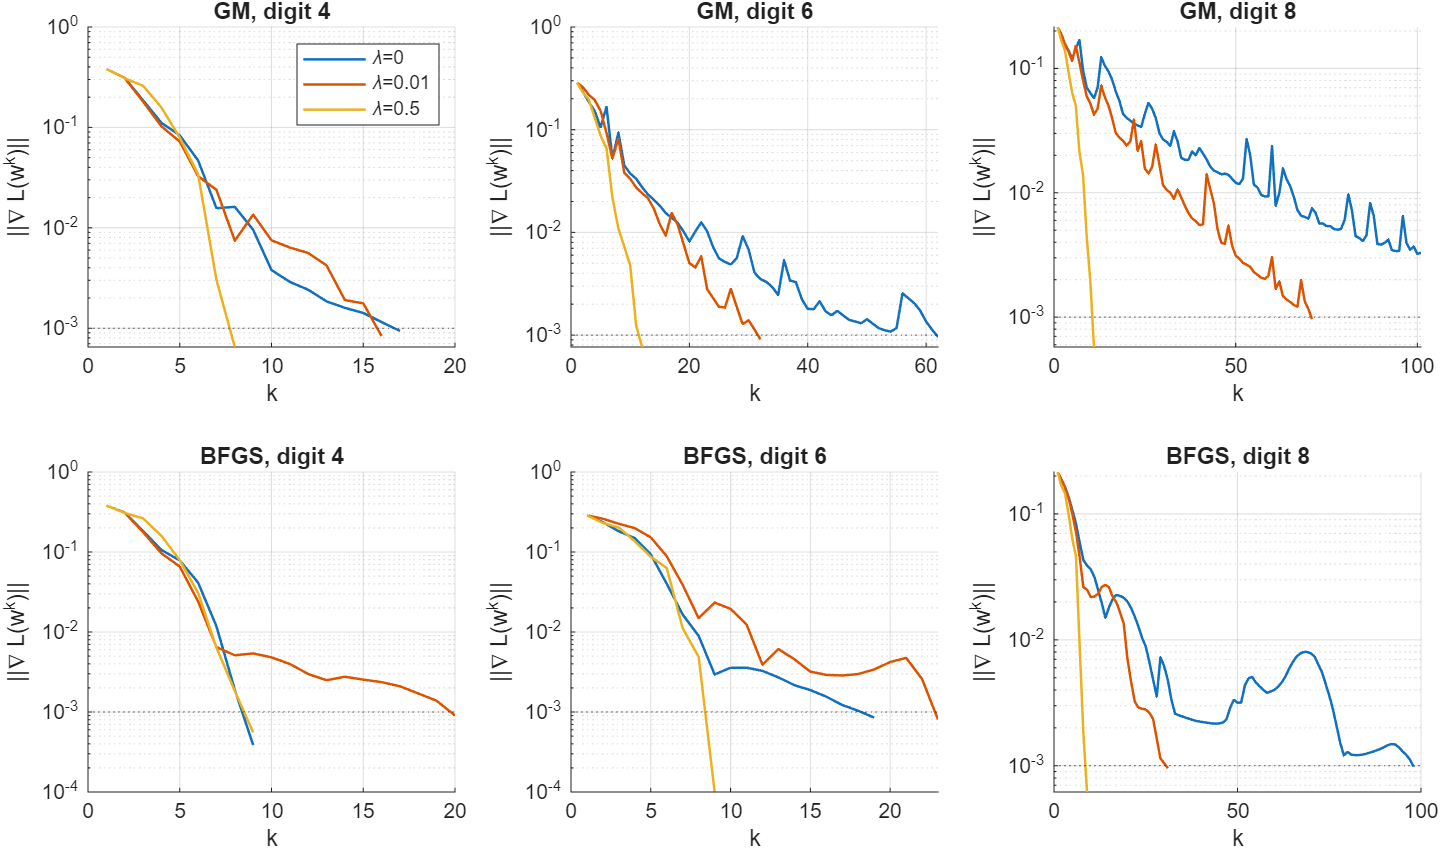
\includegraphics[width=\linewidth]{fig_rk_lambda.png}
  \caption{Gradient norm $\|\nabla\tilde L(w^k)\|$ of GM (top) and BFGS (bottom) on digits 4, 6 and 8, for $\lambda=0$ (blue), $0.01$ (red) and $0.5$ (yellow). The dotted line is the tolerance $10^{-3}$.}
  \label{fig:rklambda}
\end{figure}

\textbf{GM.} The average reduction of the gradient norm per iteration, $(\|\nabla\tilde L(w^{K+1})\|/\|\nabla\tilde L(w^1)\|)^{1/K}$, is on average 0.83 for $\lambda=0$, 0.76 for $\lambda=0.01$ and 0.50 for $\lambda=0.5$ over the ten digits. The ordering is the one predicted by the condition numbers. The observed values are smaller than the bound because the bound is a worst case, and our iterates spend part of the run far from $w^*$. The effect is clearest on digit 8 (Figure~\ref{fig:rklambda}, top right). At $\lambda=0$ the gradient norm still oscillates between $3\cdot10^{-3}$ and $10^{-2}$ after 100 iterations, at $\lambda=0.01$ it decreases more steadily and reaches the tolerance after 70 iterations, and at $\lambda=0.5$ it reaches the tolerance after 10 iterations.

\textbf{BFGS.} For $\lambda=0.5$, BFGS converges in 4 to 12 iterations in all 60 runs, with an average reduction of 0.44 per iteration and a last ratio $r_k$ between 0.02 and 0.34. For $\lambda=0.01$ the average reduction is 0.78, and the median $r_k$ over the last five iterations is 0.87. As for $\lambda=0$ (Section~\ref{sec:local}), we do not see a superlinear phase before the tolerance stops the run.

\textbf{GM against BFGS.} At $\lambda=0$, BFGS needed fewer iterations than GM on all ten digits (mean over the six generator states). At $\lambda=0.5$ this is still the case (6.8 against 9.2 iterations on average). At $\lambda=0.01$, however, BFGS needed fewer iterations only on digits 3, 8, 9 and 0, the four digits with the largest $\kappa(\nabla^2\tilde L(w^*))$ (47 to 69). On the other six digits GM was faster. The largest difference is on digit 7, with 16.2 iterations for GM and 24.7 for BFGS, where $\kappa=21$. On digit 8 the opposite holds, with 69.8 iterations for GM and 29.3 for BFGS. Our explanation is that BFGS mainly helps when the problem is badly conditioned. When $\kappa$ is small, GM is already fast. BFGS starts with $H_1=I$, the same step as GM, and needs several iterations to build a useful approximation of the inverse Hessian. During these iterations its direction deviates from $-\nabla\tilde L$ ($\cos\theta_k$ down to 0.25--0.45 for $\lambda=0.01$) without yet pointing more directly at the minimum. We did not test this explanation, for example with a scaled initial matrix $H_1$.

\textbf{Time.} The time per iteration does not depend on $\lambda$: 0.053 to 0.059\,s per iteration for both GM and BFGS and all three values (total time divided by total iterations). This is expected, since the regularization term only adds $O(n)$ operations to the loss and the gradient. The total time therefore follows the number of iterations, and for GM falls from 3.18\,s to 1.62\,s and 0.50\,s. SGM needs 11 epochs on average for both $\lambda>0$ and takes 0.24 to 0.26\,s, so $\lambda$ has no systematic effect on its run time.

\subsection{Accuracy}\label{sec:lambdaacc}

Table~\ref{tab:acclambda} gives the mean accuracies and the number of test errors, split into false negatives (target images that were rejected) and false positives (other images that were accepted).

\begin{table}[h]
\centering
\small
\setlength{\tabcolsep}{4pt}
\begin{tabular}{l ccc ccc ccc}
\toprule
 & \multicolumn{3}{c}{GM} & \multicolumn{3}{c}{BFGS} & \multicolumn{3}{c}{SGM} \\
\cmidrule(lr){2-4}\cmidrule(lr){5-7}\cmidrule(lr){8-10}
$\lambda$ & 0 & 0.01 & 0.5 & 0 & 0.01 & 0.5 & 0 & 0.01 & 0.5 \\
\midrule
Mean $\tilde L^*$ & 0.0074 & 0.0495 & 0.197 & 0.0065 & 0.0495 & 0.197 & 0.0072 & 0.0589 & 0.295 \\
Mean train acc.\ [\%] & 99.22 & 99.15 & 92.96 & 99.20 & 99.15 & 92.97 & 99.08 & 97.84 & 56.71 \\
Mean test acc.\ [\%] & 99.14 & 99.10 & 87.56 & 98.96 & 99.10 & 87.58 & 99.30 & 99.24 & 91.68 \\
Min test acc.\ [\%] & 96.6 & 96.2 & 64.4 & 96.4 & 96.2 & 64.2 & 97.4 & 98.0 & 89.6 \\
False negatives (of 500) & 5 & 6 & 0 & 6 & 6 & 0 & 8 & 27 & 416 \\
False positives (of 4500) & 38 & 39 & 622 & 46 & 39 & 621 & 27 & 11 & 0 \\
\bottomrule
\end{tabular}
\caption{Accuracy for the three values of $\lambda$, over the ten digits. The test errors are summed over the ten test sets of 500 images, which together contain 500 target and 4500 non-target images. The mean test accuracy of the always-negative classifier is 90.0\%.}
\label{tab:acclambda}
\end{table}

\textbf{$\lambda=0.01$.} The accuracy is practically the same as for $\lambda=0$: the mean test accuracy is 99.10\% for both GM and BFGS, against 99.14\% and 98.96\% without regularization, and the mean training accuracy decreases by less than 0.1 points. On single digits the test accuracy changes by at most 5 images (1 percentage point), and the changes go in both directions. Regularization is meant to reduce overfitting, and at $\lambda=0$ there was little to reduce: the network has only 35 weights for 5000 training samples, and the training and test accuracies were already similar (Section~\ref{sec:acc}). The main effect of $\lambda=0.01$ on accuracy is that GM and BFGS now return the same classifier. At $\lambda=0$ their test accuracies differed by up to 4 images on a digit, at $\lambda=0.01$ they are identical on all ten digits, because both methods find the same minimizer.

SGM behaves differently at $\lambda=0.01$. Its mean training accuracy drops to 97.84\% (93.0\% on digit 8 and 95.3\% on digit 3), while its test accuracy stays at 99.24\%. Its errors move towards false negatives (27 false negatives and 11 false positives, against 8 and 27 at $\lambda=0$). Since SGM selects its weights on the test loss and the test set is 90\% non-target, weights that reject doubtful images are favoured. The test accuracy of SGM should therefore again be read as slightly optimistic.

\textbf{$\lambda=0.5$: GM and BFGS.} Strong regularization makes the classifier clearly worse. The mean test accuracy falls to 87.6\%, which is below the 90.0\% of a classifier that always answers ``not the target''. On digit 8 it is only 64.4\%. All 622 test errors are false positives: no target image is missed, but up to 179 of the 458 non-target images are accepted on digit 8 (true negative rate 61\%). Since the test images are the same for every target, the true digit of each test image is known from the labels of the ten test sets. For target 8, 173 of the 178 false positives are 0s, 3s, 6s and 9s (45, 52, 34 and 42). For target 9 they are 0s, 3s and 8s, and for target 3 they are 2s, 8s and 9s. These are the digits whose $7\times5$ pattern overlaps most with the target (Section~\ref{sec:acc}).

We explain this as follows. With $\lambda=0.5$ the penalty dominates and $\|w^*\|\le0.44$. For small $w$, the optimality condition $\nabla L(w^*)+\lambda w^*=0$ gives $w^*\approx-\frac1\lambda\nabla L(0)$, and since $y(x,0)=\frac12$,
\[
  -\nabla L(0)=\frac{1}{4p}\sum_{j=1}^{p}(2y_j^{TR}-1)\,\sigma(x_j^{TR})\approx\frac18\left(\bar\sigma_{\text{target}}-\bar\sigma_{\text{other}}\right),
\]
where $\bar\sigma$ is the mean of $\sigma(x_j^{TR})$ over the target and the non-target images (the training set is balanced). The weights are then roughly the difference between the average target image and the average other image. Indeed, the cosine between $w^*$ and $-\nabla L(0)$ is 0.90 to 0.999 for $\lambda=0.5$, against 0.68 to 0.99 for $\lambda=0$. Such a template gives a positive score to every image that lights most of the target's pixels, which explains the false positives on the overlapping digits. With smaller $\lambda$ the weights can grow, and large negative weights can be put on the few pixels that separate, for example, an 8 from a 0. Because all errors are false positives, the test accuracy (90\% negatives) is lower than the training accuracy (50\% negatives): 87.6\% against 93.0\%. This gap is caused by the different class balance and is not a sign of overfitting.

\textbf{$\lambda=0.5$: SGM.} SGM fails in the opposite way. On 7 of the 10 digits it accepts no image at all (and only 3 on digit 7), so its test accuracy equals the always-negative baseline (for example 89.6\% on digit 3) and its training accuracy is about 50\%. Its final training loss (0.21--0.42) is higher than that of GM and BFGS (0.17--0.22), and on six digits higher than $\tilde L(0)=0.25$, the loss of the starting point. We see the following reason. The SGM update can be written as
\[
  w^{k+1}=(1-\alpha_k\lambda)\,w^k-\alpha_k\nabla L_{\mathcal B}(w^k).
\]
With $\alpha_0=2$ and $\lambda=0.5$, the factor $1-\alpha_k\lambda$ is 0 at the first iteration and at most 0.3 during the epochs in which the returned weights were found (best epoch 2 to 9, so $k\le4500$ and $\alpha_k\ge1.4$). Each step therefore keeps at most 30\% of the previous weights, and $w^k$ is determined mainly by the gradients of the last few minibatches of 10 images. The averaging of the noisy minibatch gradients, which SGM relies on, does not happen. The cosine between the SGM weights and $-\nabla L(0)$ is between $-0.24$ and $0.86$, so the SGM weights do not have the direction of the regularized minimizer. Early stopping on a test set with 90\% non-target images then selects the epoch with the lowest test loss, which in these runs is a classifier that rejects everything. For $\lambda=0.01$ the factor is at least 0.98 and this problem does not occur. A step size scaled with $\lambda$ (for example $\alpha_0\lambda\ll1$) would probably avoid it, but we did not test this.

\textbf{Across digits.} The order of difficulty of the digits does not change with $\lambda$. Digit 8 has the lowest test accuracy for every $\lambda$ for GM and BFGS (96.2\% at $\lambda=0.01$ and 64.4\% at $\lambda=0.5$), followed by 9 and 3 at $\lambda=0.5$ (74.6\% and 81.0\%). Digits 1 and 4 keep a test accuracy of 99.8\% to 100\% even at $\lambda=0.5$. Presumably their patterns differ enough from the other digits that a template of the average image is enough to recognise them.

\section{Conclusion}\label{sec:conclusion}

The three combinations with $\lambda=0.5$ can be excluded on accuracy alone. With $\lambda=0.5$, GM and BFGS are below the always-negative baseline on average (87.6\%), and SGM recognises no target images on seven digits. With $\lambda=0$ and $\lambda=0.01$ all three methods reach about 99\% test accuracy, and the differences between them are a few test images per digit, within the noise of a single test set. The choice is therefore decided by convergence.

We consider \textbf{BFGS with $\lambda=0.01$} the best combination. Its mean test accuracy is 99.10\%, the same as GM and within the noise of the best value in Table~\ref{tab:acclambda}. It converged on all ten digits in at most 31 iterations (at most 38 over all six generator states) and 1.37\,s on average. Compared with $\lambda=0$, the regularization makes the problem better posed. The iterates are bounded, the solution is a strict minimizer that GM and BFGS both find, the line search satisfies the strong Wolfe conditions at every iteration, and $\kappa(H_k)$ stays below $1.2\cdot10^{2}$ instead of reaching $10^{6}$. Compared with GM at the same $\lambda$, BFGS gives the same classifier, needs 15\% less time on average and is much faster on the hardest digit, 8 (30 against 70 iterations). GM needs fewer iterations on the six easier digits, so the advantage of BFGS comes from the hard digits.

SGM with $\lambda=0.01$ (or $\lambda=0$) is the fastest option, about 5.7 times faster than BFGS (0.24\,s on average), with a mean test accuracy of 99.24\%. We do not choose it because its test accuracy is measured on the same set that selects its weights, its training accuracy is lower (97.84\%), and its solutions are not stationary points. It also fails completely at $\lambda=0.5$ with the step sizes used here. For a training set much larger than our $p=5000$, the cost of the full gradient would grow with $p$ while the cost of an SGM step would not, and SGM would become the preferable method.
 before \end{document}.
% Needs fig_rk_lambda.png (made by Code/uonn/uo_nn_lambda_analysis.m).

\section{Effect of regularization}\label{sec:lambdapos}

We now compare the runs with $\lambda\in\{0,\,0.01,\,0.5\}$. As in Section~\ref{sec:lambda0}, the iterations, losses, times and accuracies come from the batch, and the other quantities from \texttt{uo\_nn\_\allowbreak lambda\_\allowbreak analysis.m} (Section~1, Experimental setup). Since the number of GM and BFGS iterations depends on the state of the random generator used by the line search, we also give the mean over the batch run and the five repetitions with other states when we compare iteration counts.

\subsection{Global convergence}\label{sec:lambdaglobal}

\textbf{Theory.} For $\lambda>0$ the objective has a property that it lacks for $\lambda=0$: since the data term is non-negative, $\tilde L(w)\ge\frac{\lambda}{2}\|w\|^2$, so $\tilde L(w)\to\infty$ when $\|w\|\to\infty$. GM and BFGS with a Wolfe line search decrease $\tilde L$ at every iteration, so all iterates stay in the level set $\{w:\tilde L(w)\le\tilde L(w^1)=0.25\}$, which gives
\[
  \|w^k\|\le\sqrt{0.5/\lambda}\;=\;7.1 \text{ for } \lambda=0.01,\qquad 1.0 \text{ for } \lambda=0.5 .
\]
The iterates are therefore bounded and the minimum of $\tilde L$ is attained. For $\lambda=0$ there is no such bound. The loss can keep decreasing while $\|w\|$ grows, because the sigmoid only approaches 0 and 1 for arguments of growing size. In addition, $\lambda I$ is added to the Hessian, $\nabla^2\tilde L=\nabla^2 L+\lambda I$, which raises its smallest eigenvalue by $\lambda$ and lowers its condition number. Both effects should make convergence easier as $\lambda$ grows.

\textbf{Observations.} Table~\ref{tab:convlambda} summarizes the convergence for the three values of $\lambda$.

\begin{table}[h]
\centering
\small
\setlength{\tabcolsep}{3pt}
\begin{tabular}{l ccc ccc ccc}
\toprule
 & \multicolumn{3}{c}{GM} & \multicolumn{3}{c}{BFGS} & \multicolumn{3}{c}{SGM} \\
\cmidrule(lr){2-4}\cmidrule(lr){5-7}\cmidrule(lr){8-10}
$\lambda$ & 0 & 0.01 & 0.5 & 0 & 0.01 & 0.5 & 0 & 0.01 & 0.5 \\
\midrule
Mean iter.\ / epochs & 57.3 & 29.5 & 9.4 & 31.6 & 24.2 & 8.0 & 18.3 & 11.2 & 11.3 \\
Max iter.\ / epochs & 100 & 70 & 13 & 97 & 31 & 9 & 100 & 16 & 14 \\
Not converged & 2 & 0 & 0 & 0 & 0 & 0 & 1 & 0 & 0 \\
Mean, 6 gen.\ states & 57.6 & 31.5 & 9.2 & 33.2 & 25.6 & 6.8 & -- & -- & -- \\
Mean $t$ [s] & 3.18 & 1.62 & 0.50 & 1.78 & 1.37 & 0.47 & 0.33 & 0.24 & 0.26 \\
$\|w^*\|$ & 3.6--6.4 & 1.8--2.4 & .29--.44 & 4.6--35 & 1.8--2.5 & .29--.44 & 4.7--9.6 & 1.8--2.7 & .33--.58 \\
Max $\|\nabla\tilde L(w^*)\|$ & $2.8{\cdot}10^{-3}$ & $9.9{\cdot}10^{-4}$ & $7.7{\cdot}10^{-4}$ & $9.9{\cdot}10^{-4}$ & $9.9{\cdot}10^{-4}$ & $7.4{\cdot}10^{-4}$ & $2.5{\cdot}10^{-2}$ & 0.22 & 0.62 \\
\bottomrule
\end{tabular}
\caption{Convergence for the three values of $\lambda$, over the ten digits. Iterations for GM and BFGS, epochs for SGM. ``Not converged'' means the iteration limit was reached with $\|\nabla\tilde L\|>10^{-3}$ (GM, BFGS) or the 100-epoch limit was reached (SGM). The ``6 generator states'' row is the mean over the batch run and the five repetitions with \texttt{rng(1)}--\texttt{rng(5)}.}
\label{tab:convlambda}
\end{table}

\begin{itemize}
  \item \textbf{GM} converges on all digits for both $\lambda>0$, while at $\lambda=0$ it reached the 100-iteration limit on digits 3 and 8. The mean number of iterations halves from $\lambda=0$ to $\lambda=0.01$ and drops by a further factor of three at $\lambda=0.5$. In the repetitions with other generator states, GM at $\lambda=0$ reached the limit in 18 of 60 runs (always on digits 3, 8 and 9), and for $\lambda>0$ it never needed more than 78 iterations.
  \item \textbf{BFGS} converged on all digits for every $\lambda$, but the worst case improves strongly: from 97 iterations at $\lambda=0$ to 31 and 9. The quantities in the global convergence conditions behave in the same way. Over all BFGS iterations, $\kappa(H_k)$ reached up to $1.6\cdot10^{6}$ for $\lambda=0$, but only $1.2\cdot10^{2}$ for $\lambda=0.01$ and $3.3$ for $\lambda=0.5$. The smallest $\cos\theta_k$ was $0.005$, $0.25$ and $0.94$. For $\lambda>0$ the direction is therefore well away from orthogonal to the gradient, and the condition of Section~\ref{sec:global} holds with a large margin. The line search found a strong Wolfe step in every BFGS iteration for $\lambda>0$. For GM it did so in every iteration except 6 of the 162 iterations on digits 3, 8 and 9 with $\lambda=0.01$.
  \item \textbf{The solution becomes well defined.} At $\lambda=0$, GM and BFGS stop at different points: $\|w^*\|$ is 6.0 for GM and 35 for BFGS on digit 2, and the two final losses differ on every digit (Table~\ref{tab:acc}). The Hessian at the BFGS solutions has small negative eigenvalues on six digits (down to $-5.6\cdot10^{-4}$), so these points are not strict minimizers. For $\lambda>0$, GM and BFGS give the same $\tilde L^*$ to three digits and $\|w^*\|$ within 0.03 on every digit, and the smallest Hessian eigenvalue is 0.011--0.013 for $\lambda=0.01$ and 0.51 for $\lambda=0.5$, that is, about $\lambda$. The observed $\|w^*\|$ is also well inside the bound $\sqrt{0.5/\lambda}$ above.
  \item \textbf{SGM} stopped early on all 20 runs with $\lambda>0$, after 6 to 16 epochs, so in the sense of Section~\ref{sec:global} it converged on every digit. The returned points are, however, further from stationary as $\lambda$ grows: $\|\nabla\tilde L(w^*)\|$ on the full training set is at most $2.5\cdot10^{-2}$ for $\lambda=0$, between $2.3\cdot10^{-2}$ and $0.22$ for $\lambda=0.01$, and between 0.35 and 0.62 for $\lambda=0.5$. The reason for $\lambda=0.5$ is discussed in Section~\ref{sec:lambdaacc}.
\end{itemize}

In summary, regularization makes the global convergence of GM and BFGS easier, both in theory (bounded level sets, a positive definite Hessian at the solution) and in the experiments (no iteration limit reached, well-conditioned $H_k$). It does not help SGM in the same way, because its run length is set by early stopping and not by the gradient.

\subsection{Local convergence and speed}\label{sec:lambdalocal}

\textbf{Conditioning.} The condition number of the Hessian at the solution, $\kappa(\nabla^2\tilde L(w^*))$, is $1.7\cdot10^{2}$--$3.0\cdot10^{2}$ at the GM solutions for $\lambda=0$, 17--69 for $\lambda=0.01$ and 3.1--4.1 for $\lambda=0.5$. For GM the theory predicts a linear rate that gets worse as $\kappa$ grows. With an exact line search the bound on the reduction of $\tilde L-\tilde L^*$ per iteration is $\left(\frac{\kappa-1}{\kappa+1}\right)^2$, which is 0.98, 0.92 and 0.36 for $\kappa=250$, 50 and 4. Figure~\ref{fig:rklambda} shows the gradient norm for digits 4, 6 and 8.

\begin{figure}[h]
  \centering
  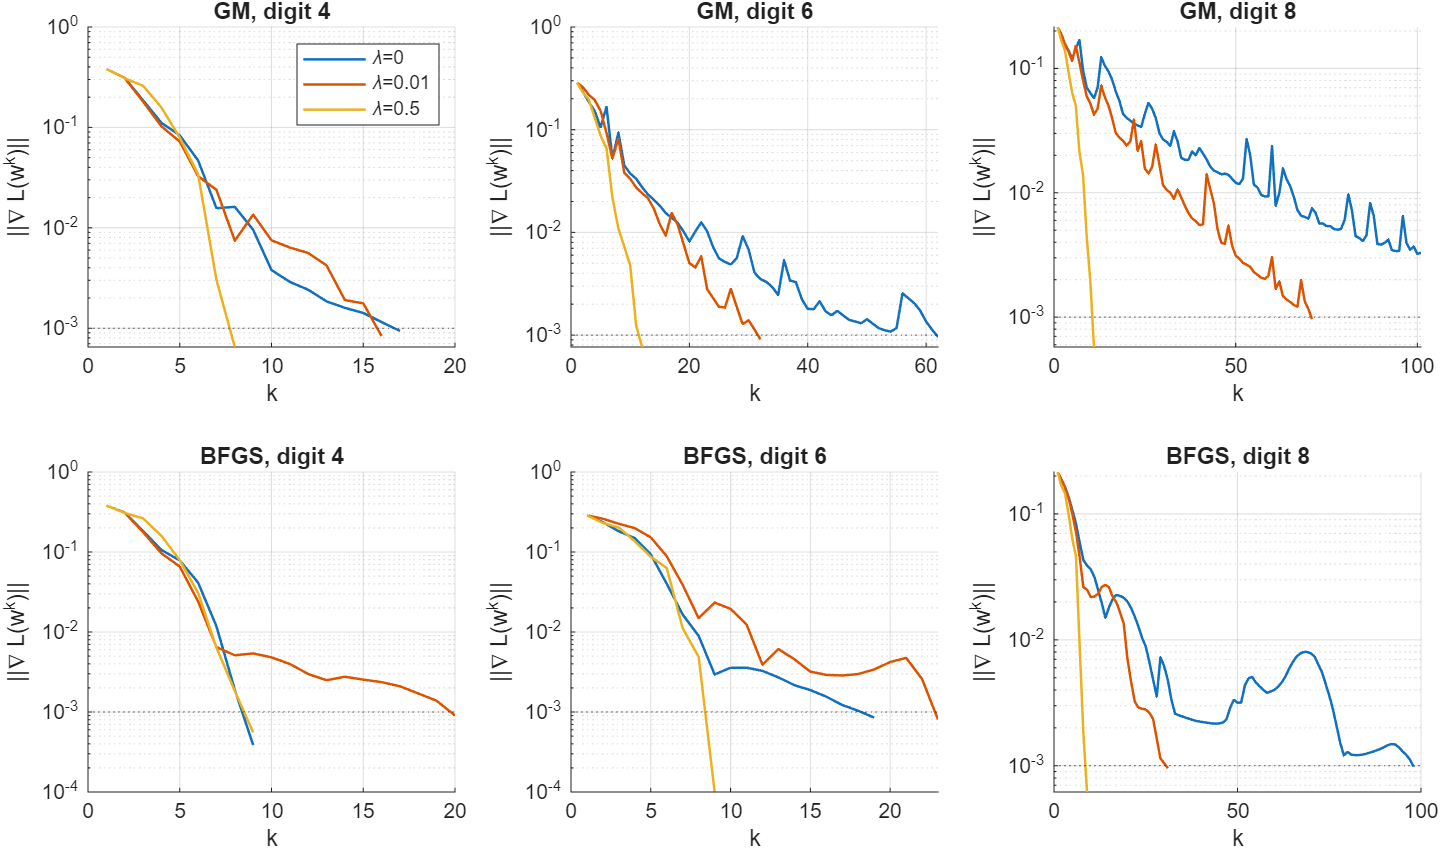
\includegraphics[width=\linewidth]{fig_rk_lambda.png}
  \caption{Gradient norm $\|\nabla\tilde L(w^k)\|$ of GM (top) and BFGS (bottom) on digits 4, 6 and 8, for $\lambda=0$ (blue), $0.01$ (red) and $0.5$ (yellow). The dotted line is the tolerance $10^{-3}$.}
  \label{fig:rklambda}
\end{figure}

\textbf{GM.} The average reduction of the gradient norm per iteration, $(\|\nabla\tilde L(w^{K+1})\|/\|\nabla\tilde L(w^1)\|)^{1/K}$, is on average 0.83 for $\lambda=0$, 0.76 for $\lambda=0.01$ and 0.50 for $\lambda=0.5$ over the ten digits. The ordering is the one predicted by the condition numbers. The observed values are smaller than the bound because the bound is a worst case, and our iterates spend part of the run far from $w^*$. The effect is clearest on digit 8 (Figure~\ref{fig:rklambda}, top right). At $\lambda=0$ the gradient norm still oscillates between $3\cdot10^{-3}$ and $10^{-2}$ after 100 iterations, at $\lambda=0.01$ it decreases more steadily and reaches the tolerance after 70 iterations, and at $\lambda=0.5$ it reaches the tolerance after 10 iterations.

\textbf{BFGS.} For $\lambda=0.5$, BFGS converges in 4 to 12 iterations in all 60 runs, with an average reduction of 0.44 per iteration and a last ratio $r_k$ between 0.02 and 0.34. For $\lambda=0.01$ the average reduction is 0.78, and the median $r_k$ over the last five iterations is 0.87. As for $\lambda=0$ (Section~\ref{sec:local}), we do not see a superlinear phase before the tolerance stops the run.

\textbf{GM against BFGS.} At $\lambda=0$, BFGS needed fewer iterations than GM on all ten digits (mean over the six generator states). At $\lambda=0.5$ this is still the case (6.8 against 9.2 iterations on average). At $\lambda=0.01$, however, BFGS needed fewer iterations only on digits 3, 8, 9 and 0, the four digits with the largest $\kappa(\nabla^2\tilde L(w^*))$ (47 to 69). On the other six digits GM was faster. The largest difference is on digit 7, with 16.2 iterations for GM and 24.7 for BFGS, where $\kappa=21$. On digit 8 the opposite holds, with 69.8 iterations for GM and 29.3 for BFGS. Our explanation is that BFGS mainly helps when the problem is badly conditioned. When $\kappa$ is small, GM is already fast. BFGS starts with $H_1=I$, the same step as GM, and needs several iterations to build a useful approximation of the inverse Hessian. During these iterations its direction deviates from $-\nabla\tilde L$ ($\cos\theta_k$ down to 0.25--0.45 for $\lambda=0.01$) without yet pointing more directly at the minimum. We did not test this explanation, for example with a scaled initial matrix $H_1$.

\textbf{Time.} The time per iteration does not depend on $\lambda$: 0.053 to 0.059\,s per iteration for both GM and BFGS and all three values (total time divided by total iterations). This is expected, since the regularization term only adds $O(n)$ operations to the loss and the gradient. The total time therefore follows the number of iterations, and for GM falls from 3.18\,s to 1.62\,s and 0.50\,s. SGM needs 11 epochs on average for both $\lambda>0$ and takes 0.24 to 0.26\,s, so $\lambda$ has no systematic effect on its run time.

\subsection{Accuracy}\label{sec:lambdaacc}

Table~\ref{tab:acclambda} gives the mean accuracies and the number of test errors, split into false negatives (target images that were rejected) and false positives (other images that were accepted).

\begin{table}[h]
\centering
\small
\setlength{\tabcolsep}{4pt}
\begin{tabular}{l ccc ccc ccc}
\toprule
 & \multicolumn{3}{c}{GM} & \multicolumn{3}{c}{BFGS} & \multicolumn{3}{c}{SGM} \\
\cmidrule(lr){2-4}\cmidrule(lr){5-7}\cmidrule(lr){8-10}
$\lambda$ & 0 & 0.01 & 0.5 & 0 & 0.01 & 0.5 & 0 & 0.01 & 0.5 \\
\midrule
Mean $\tilde L^*$ & 0.0074 & 0.0495 & 0.197 & 0.0065 & 0.0495 & 0.197 & 0.0072 & 0.0589 & 0.295 \\
Mean train acc.\ [\%] & 99.22 & 99.15 & 92.96 & 99.20 & 99.15 & 92.97 & 99.08 & 97.84 & 56.71 \\
Mean test acc.\ [\%] & 99.14 & 99.10 & 87.56 & 98.96 & 99.10 & 87.58 & 99.30 & 99.24 & 91.68 \\
Min test acc.\ [\%] & 96.6 & 96.2 & 64.4 & 96.4 & 96.2 & 64.2 & 97.4 & 98.0 & 89.6 \\
False negatives (of 500) & 5 & 6 & 0 & 6 & 6 & 0 & 8 & 27 & 416 \\
False positives (of 4500) & 38 & 39 & 622 & 46 & 39 & 621 & 27 & 11 & 0 \\
\bottomrule
\end{tabular}
\caption{Accuracy for the three values of $\lambda$, over the ten digits. The test errors are summed over the ten test sets of 500 images, which together contain 500 target and 4500 non-target images. The mean test accuracy of the always-negative classifier is 90.0\%.}
\label{tab:acclambda}
\end{table}

\textbf{$\lambda=0.01$.} The accuracy is practically the same as for $\lambda=0$: the mean test accuracy is 99.10\% for both GM and BFGS, against 99.14\% and 98.96\% without regularization, and the mean training accuracy decreases by less than 0.1 points. On single digits the test accuracy changes by at most 5 images (1 percentage point), and the changes go in both directions. Regularization is meant to reduce overfitting, and at $\lambda=0$ there was little to reduce: the network has only 35 weights for 5000 training samples, and the training and test accuracies were already similar (Section~\ref{sec:acc}). The main effect of $\lambda=0.01$ on accuracy is that GM and BFGS now return the same classifier. At $\lambda=0$ their test accuracies differed by up to 4 images on a digit, at $\lambda=0.01$ they are identical on all ten digits, because both methods find the same minimizer.

SGM behaves differently at $\lambda=0.01$. Its mean training accuracy drops to 97.84\% (93.0\% on digit 8 and 95.3\% on digit 3), while its test accuracy stays at 99.24\%. Its errors move towards false negatives (27 false negatives and 11 false positives, against 8 and 27 at $\lambda=0$). Since SGM selects its weights on the test loss and the test set is 90\% non-target, weights that reject doubtful images are favoured. The test accuracy of SGM should therefore again be read as slightly optimistic.

\textbf{$\lambda=0.5$: GM and BFGS.} Strong regularization makes the classifier clearly worse. The mean test accuracy falls to 87.6\%, which is below the 90.0\% of a classifier that always answers ``not the target''. On digit 8 it is only 64.4\%. All 622 test errors are false positives: no target image is missed, but up to 179 of the 458 non-target images are accepted on digit 8 (true negative rate 61\%). Since the test images are the same for every target, the true digit of each test image is known from the labels of the ten test sets. For target 8, 173 of the 178 false positives are 0s, 3s, 6s and 9s (45, 52, 34 and 42). For target 9 they are 0s, 3s and 8s, and for target 3 they are 2s, 8s and 9s. These are the digits whose $7\times5$ pattern overlaps most with the target (Section~\ref{sec:acc}).

We explain this as follows. With $\lambda=0.5$ the penalty dominates and $\|w^*\|\le0.44$. For small $w$, the optimality condition $\nabla L(w^*)+\lambda w^*=0$ gives $w^*\approx-\frac1\lambda\nabla L(0)$, and since $y(x,0)=\frac12$,
\[
  -\nabla L(0)=\frac{1}{4p}\sum_{j=1}^{p}(2y_j^{TR}-1)\,\sigma(x_j^{TR})\approx\frac18\left(\bar\sigma_{\text{target}}-\bar\sigma_{\text{other}}\right),
\]
where $\bar\sigma$ is the mean of $\sigma(x_j^{TR})$ over the target and the non-target images (the training set is balanced). The weights are then roughly the difference between the average target image and the average other image. Indeed, the cosine between $w^*$ and $-\nabla L(0)$ is 0.90 to 0.999 for $\lambda=0.5$, against 0.68 to 0.99 for $\lambda=0$. Such a template gives a positive score to every image that lights most of the target's pixels, which explains the false positives on the overlapping digits. With smaller $\lambda$ the weights can grow, and large negative weights can be put on the few pixels that separate, for example, an 8 from a 0. Because all errors are false positives, the test accuracy (90\% negatives) is lower than the training accuracy (50\% negatives): 87.6\% against 93.0\%. This gap is caused by the different class balance and is not a sign of overfitting.

\textbf{$\lambda=0.5$: SGM.} SGM fails in the opposite way. On 7 of the 10 digits it accepts no image at all (and only 3 on digit 7), so its test accuracy equals the always-negative baseline (for example 89.6\% on digit 3) and its training accuracy is about 50\%. Its final training loss (0.21--0.42) is higher than that of GM and BFGS (0.17--0.22), and on six digits higher than $\tilde L(0)=0.25$, the loss of the starting point. We see the following reason. The SGM update can be written as
\[
  w^{k+1}=(1-\alpha_k\lambda)\,w^k-\alpha_k\nabla L_{\mathcal B}(w^k).
\]
With $\alpha_0=2$ and $\lambda=0.5$, the factor $1-\alpha_k\lambda$ is 0 at the first iteration and at most 0.3 during the epochs in which the returned weights were found (best epoch 2 to 9, so $k\le4500$ and $\alpha_k\ge1.4$). Each step therefore keeps at most 30\% of the previous weights, and $w^k$ is determined mainly by the gradients of the last few minibatches of 10 images. The averaging of the noisy minibatch gradients, which SGM relies on, does not happen. The cosine between the SGM weights and $-\nabla L(0)$ is between $-0.24$ and $0.86$, so the SGM weights do not have the direction of the regularized minimizer. Early stopping on a test set with 90\% non-target images then selects the epoch with the lowest test loss, which in these runs is a classifier that rejects everything. For $\lambda=0.01$ the factor is at least 0.98 and this problem does not occur. A step size scaled with $\lambda$ (for example $\alpha_0\lambda\ll1$) would probably avoid it, but we did not test this.

\textbf{Across digits.} The order of difficulty of the digits does not change with $\lambda$. Digit 8 has the lowest test accuracy for every $\lambda$ for GM and BFGS (96.2\% at $\lambda=0.01$ and 64.4\% at $\lambda=0.5$), followed by 9 and 3 at $\lambda=0.5$ (74.6\% and 81.0\%). Digits 1 and 4 keep a test accuracy of 99.8\% to 100\% even at $\lambda=0.5$. Presumably their patterns differ enough from the other digits that a template of the average image is enough to recognise them.

\section{Conclusion}\label{sec:conclusion}

The three combinations with $\lambda=0.5$ can be excluded on accuracy alone. With $\lambda=0.5$, GM and BFGS are below the always-negative baseline on average (87.6\%), and SGM recognises no target images on seven digits. With $\lambda=0$ and $\lambda=0.01$ all three methods reach about 99\% test accuracy, and the differences between them are a few test images per digit, within the noise of a single test set. The choice is therefore decided by convergence.

We consider \textbf{BFGS with $\lambda=0.01$} the best combination. Its mean test accuracy is 99.10\%, the same as GM and within the noise of the best value in Table~\ref{tab:acclambda}. It converged on all ten digits in at most 31 iterations (at most 38 over all six generator states) and 1.37\,s on average. Compared with $\lambda=0$, the regularization makes the problem better posed. The iterates are bounded, the solution is a strict minimizer that GM and BFGS both find, the line search satisfies the strong Wolfe conditions at every iteration, and $\kappa(H_k)$ stays below $1.2\cdot10^{2}$ instead of reaching $10^{6}$. Compared with GM at the same $\lambda$, BFGS gives the same classifier, needs 15\% less time on average and is much faster on the hardest digit, 8 (30 against 70 iterations). GM needs fewer iterations on the six easier digits, so the advantage of BFGS comes from the hard digits.

SGM with $\lambda=0.01$ (or $\lambda=0$) is the fastest option, about 5.7 times faster than BFGS (0.24\,s on average), with a mean test accuracy of 99.24\%. We do not choose it because its test accuracy is measured on the same set that selects its weights, its training accuracy is lower (97.84\%), and its solutions are not stationary points. It also fails completely at $\lambda=0.5$ with the step sizes used here. For a training set much larger than our $p=5000$, the cost of the full gradient would grow with $p$ while the cost of an SGM step would not, and SGM would become the preferable method.
 before \end{document}.
% Needs fig_rk_lambda.png (made by Code/uonn/uo_nn_lambda_analysis.m).

\section{Effect of regularization}\label{sec:lambdapos}

We now compare the runs with $\lambda\in\{0,\,0.01,\,0.5\}$. As in Section~\ref{sec:lambda0}, the iterations, losses, times and accuracies come from the batch, and the other quantities from \texttt{uo\_nn\_\allowbreak lambda\_\allowbreak analysis.m} (Section~1, Experimental setup). Since the number of GM and BFGS iterations depends on the state of the random generator used by the line search, we also give the mean over the batch run and the five repetitions with other states when we compare iteration counts.

\subsection{Global convergence}\label{sec:lambdaglobal}

\textbf{Theory.} For $\lambda>0$ the objective has a property that it lacks for $\lambda=0$: since the data term is non-negative, $\tilde L(w)\ge\frac{\lambda}{2}\|w\|^2$, so $\tilde L(w)\to\infty$ when $\|w\|\to\infty$. GM and BFGS with a Wolfe line search decrease $\tilde L$ at every iteration, so all iterates stay in the level set $\{w:\tilde L(w)\le\tilde L(w^1)=0.25\}$, which gives
\[
  \|w^k\|\le\sqrt{0.5/\lambda}\;=\;7.1 \text{ for } \lambda=0.01,\qquad 1.0 \text{ for } \lambda=0.5 .
\]
The iterates are therefore bounded and the minimum of $\tilde L$ is attained. For $\lambda=0$ there is no such bound. The loss can keep decreasing while $\|w\|$ grows, because the sigmoid only approaches 0 and 1 for arguments of growing size. In addition, $\lambda I$ is added to the Hessian, $\nabla^2\tilde L=\nabla^2 L+\lambda I$, which raises its smallest eigenvalue by $\lambda$ and lowers its condition number. Both effects should make convergence easier as $\lambda$ grows.

\textbf{Observations.} Table~\ref{tab:convlambda} summarizes the convergence for the three values of $\lambda$.

\begin{table}[h]
\centering
\small
\setlength{\tabcolsep}{3pt}
\begin{tabular}{l ccc ccc ccc}
\toprule
 & \multicolumn{3}{c}{GM} & \multicolumn{3}{c}{BFGS} & \multicolumn{3}{c}{SGM} \\
\cmidrule(lr){2-4}\cmidrule(lr){5-7}\cmidrule(lr){8-10}
$\lambda$ & 0 & 0.01 & 0.5 & 0 & 0.01 & 0.5 & 0 & 0.01 & 0.5 \\
\midrule
Mean iter.\ / epochs & 57.3 & 29.5 & 9.4 & 31.6 & 24.2 & 8.0 & 18.3 & 11.2 & 11.3 \\
Max iter.\ / epochs & 100 & 70 & 13 & 97 & 31 & 9 & 100 & 16 & 14 \\
Not converged & 2 & 0 & 0 & 0 & 0 & 0 & 1 & 0 & 0 \\
Mean, 6 gen.\ states & 57.6 & 31.5 & 9.2 & 33.2 & 25.6 & 6.8 & -- & -- & -- \\
Mean $t$ [s] & 3.18 & 1.62 & 0.50 & 1.78 & 1.37 & 0.47 & 0.33 & 0.24 & 0.26 \\
$\|w^*\|$ & 3.6--6.4 & 1.8--2.4 & .29--.44 & 4.6--35 & 1.8--2.5 & .29--.44 & 4.7--9.6 & 1.8--2.7 & .33--.58 \\
Max $\|\nabla\tilde L(w^*)\|$ & $2.8{\cdot}10^{-3}$ & $9.9{\cdot}10^{-4}$ & $7.7{\cdot}10^{-4}$ & $9.9{\cdot}10^{-4}$ & $9.9{\cdot}10^{-4}$ & $7.4{\cdot}10^{-4}$ & $2.5{\cdot}10^{-2}$ & 0.22 & 0.62 \\
\bottomrule
\end{tabular}
\caption{Convergence for the three values of $\lambda$, over the ten digits. Iterations for GM and BFGS, epochs for SGM. ``Not converged'' means the iteration limit was reached with $\|\nabla\tilde L\|>10^{-3}$ (GM, BFGS) or the 100-epoch limit was reached (SGM). The ``6 generator states'' row is the mean over the batch run and the five repetitions with \texttt{rng(1)}--\texttt{rng(5)}.}
\label{tab:convlambda}
\end{table}

\begin{itemize}
  \item \textbf{GM} converges on all digits for both $\lambda>0$, while at $\lambda=0$ it reached the 100-iteration limit on digits 3 and 8. The mean number of iterations halves from $\lambda=0$ to $\lambda=0.01$ and drops by a further factor of three at $\lambda=0.5$. In the repetitions with other generator states, GM at $\lambda=0$ reached the limit in 18 of 60 runs (always on digits 3, 8 and 9), and for $\lambda>0$ it never needed more than 78 iterations.
  \item \textbf{BFGS} converged on all digits for every $\lambda$, but the worst case improves strongly: from 97 iterations at $\lambda=0$ to 31 and 9. The quantities in the global convergence conditions behave in the same way. Over all BFGS iterations, $\kappa(H_k)$ reached up to $1.6\cdot10^{6}$ for $\lambda=0$, but only $1.2\cdot10^{2}$ for $\lambda=0.01$ and $3.3$ for $\lambda=0.5$. The smallest $\cos\theta_k$ was $0.005$, $0.25$ and $0.94$. For $\lambda>0$ the direction is therefore well away from orthogonal to the gradient, and the condition of Section~\ref{sec:global} holds with a large margin. The line search found a strong Wolfe step in every BFGS iteration for $\lambda>0$. For GM it did so in every iteration except 6 of the 162 iterations on digits 3, 8 and 9 with $\lambda=0.01$.
  \item \textbf{The solution becomes well defined.} At $\lambda=0$, GM and BFGS stop at different points: $\|w^*\|$ is 6.0 for GM and 35 for BFGS on digit 2, and the two final losses differ on every digit (Table~\ref{tab:acc}). The Hessian at the BFGS solutions has small negative eigenvalues on six digits (down to $-5.6\cdot10^{-4}$), so these points are not strict minimizers. For $\lambda>0$, GM and BFGS give the same $\tilde L^*$ to three digits and $\|w^*\|$ within 0.03 on every digit, and the smallest Hessian eigenvalue is 0.011--0.013 for $\lambda=0.01$ and 0.51 for $\lambda=0.5$, that is, about $\lambda$. The observed $\|w^*\|$ is also well inside the bound $\sqrt{0.5/\lambda}$ above.
  \item \textbf{SGM} stopped early on all 20 runs with $\lambda>0$, after 6 to 16 epochs, so in the sense of Section~\ref{sec:global} it converged on every digit. The returned points are, however, further from stationary as $\lambda$ grows: $\|\nabla\tilde L(w^*)\|$ on the full training set is at most $2.5\cdot10^{-2}$ for $\lambda=0$, between $2.3\cdot10^{-2}$ and $0.22$ for $\lambda=0.01$, and between 0.35 and 0.62 for $\lambda=0.5$. The reason for $\lambda=0.5$ is discussed in Section~\ref{sec:lambdaacc}.
\end{itemize}

In summary, regularization makes the global convergence of GM and BFGS easier, both in theory (bounded level sets, a positive definite Hessian at the solution) and in the experiments (no iteration limit reached, well-conditioned $H_k$). It does not help SGM in the same way, because its run length is set by early stopping and not by the gradient.

\subsection{Local convergence and speed}\label{sec:lambdalocal}

\textbf{Conditioning.} The condition number of the Hessian at the solution, $\kappa(\nabla^2\tilde L(w^*))$, is $1.7\cdot10^{2}$--$3.0\cdot10^{2}$ at the GM solutions for $\lambda=0$, 17--69 for $\lambda=0.01$ and 3.1--4.1 for $\lambda=0.5$. For GM the theory predicts a linear rate that gets worse as $\kappa$ grows. With an exact line search the bound on the reduction of $\tilde L-\tilde L^*$ per iteration is $\left(\frac{\kappa-1}{\kappa+1}\right)^2$, which is 0.98, 0.92 and 0.36 for $\kappa=250$, 50 and 4. Figure~\ref{fig:rklambda} shows the gradient norm for digits 4, 6 and 8.

\begin{figure}[h]
  \centering
  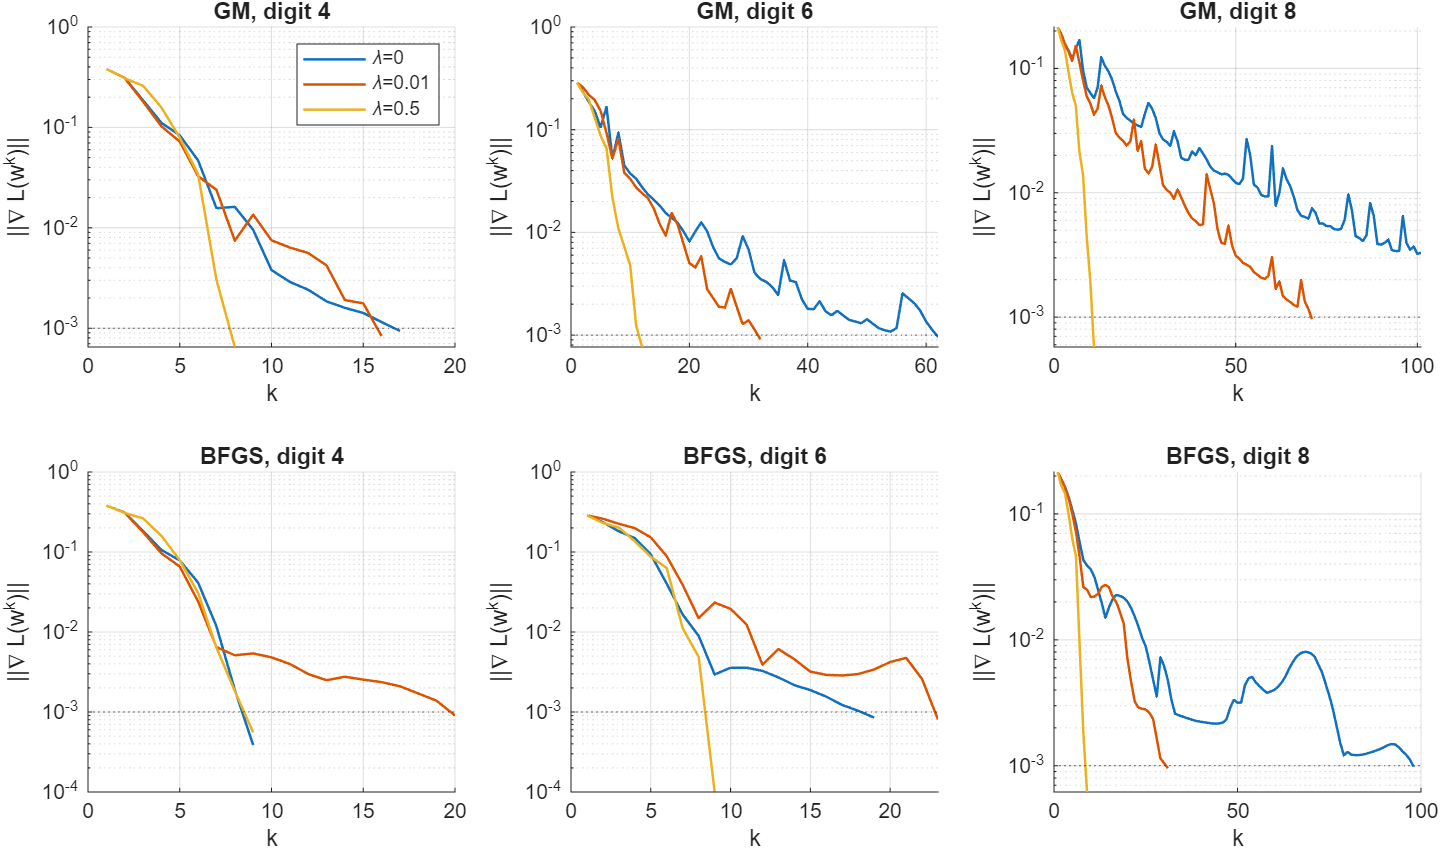
\includegraphics[width=\linewidth]{fig_rk_lambda.png}
  \caption{Gradient norm $\|\nabla\tilde L(w^k)\|$ of GM (top) and BFGS (bottom) on digits 4, 6 and 8, for $\lambda=0$ (blue), $0.01$ (red) and $0.5$ (yellow). The dotted line is the tolerance $10^{-3}$.}
  \label{fig:rklambda}
\end{figure}

\textbf{GM.} The average reduction of the gradient norm per iteration, $(\|\nabla\tilde L(w^{K+1})\|/\|\nabla\tilde L(w^1)\|)^{1/K}$, is on average 0.83 for $\lambda=0$, 0.76 for $\lambda=0.01$ and 0.50 for $\lambda=0.5$ over the ten digits. The ordering is the one predicted by the condition numbers. The observed values are smaller than the bound because the bound is a worst case, and our iterates spend part of the run far from $w^*$. The effect is clearest on digit 8 (Figure~\ref{fig:rklambda}, top right). At $\lambda=0$ the gradient norm still oscillates between $3\cdot10^{-3}$ and $10^{-2}$ after 100 iterations, at $\lambda=0.01$ it decreases more steadily and reaches the tolerance after 70 iterations, and at $\lambda=0.5$ it reaches the tolerance after 10 iterations.

\textbf{BFGS.} For $\lambda=0.5$, BFGS converges in 4 to 12 iterations in all 60 runs, with an average reduction of 0.44 per iteration and a last ratio $r_k$ between 0.02 and 0.34. For $\lambda=0.01$ the average reduction is 0.78, and the median $r_k$ over the last five iterations is 0.87. As for $\lambda=0$ (Section~\ref{sec:local}), we do not see a superlinear phase before the tolerance stops the run.

\textbf{GM against BFGS.} At $\lambda=0$, BFGS needed fewer iterations than GM on all ten digits (mean over the six generator states). At $\lambda=0.5$ this is still the case (6.8 against 9.2 iterations on average). At $\lambda=0.01$, however, BFGS needed fewer iterations only on digits 3, 8, 9 and 0, the four digits with the largest $\kappa(\nabla^2\tilde L(w^*))$ (47 to 69). On the other six digits GM was faster. The largest difference is on digit 7, with 16.2 iterations for GM and 24.7 for BFGS, where $\kappa=21$. On digit 8 the opposite holds, with 69.8 iterations for GM and 29.3 for BFGS. Our explanation is that BFGS mainly helps when the problem is badly conditioned. When $\kappa$ is small, GM is already fast. BFGS starts with $H_1=I$, the same step as GM, and needs several iterations to build a useful approximation of the inverse Hessian. During these iterations its direction deviates from $-\nabla\tilde L$ ($\cos\theta_k$ down to 0.25--0.45 for $\lambda=0.01$) without yet pointing more directly at the minimum. We did not test this explanation, for example with a scaled initial matrix $H_1$.

\textbf{Time.} The time per iteration does not depend on $\lambda$: 0.053 to 0.059\,s per iteration for both GM and BFGS and all three values (total time divided by total iterations). This is expected, since the regularization term only adds $O(n)$ operations to the loss and the gradient. The total time therefore follows the number of iterations, and for GM falls from 3.18\,s to 1.62\,s and 0.50\,s. SGM needs 11 epochs on average for both $\lambda>0$ and takes 0.24 to 0.26\,s, so $\lambda$ has no systematic effect on its run time.

\subsection{Accuracy}\label{sec:lambdaacc}

Table~\ref{tab:acclambda} gives the mean accuracies and the number of test errors, split into false negatives (target images that were rejected) and false positives (other images that were accepted).

\begin{table}[h]
\centering
\small
\setlength{\tabcolsep}{4pt}
\begin{tabular}{l ccc ccc ccc}
\toprule
 & \multicolumn{3}{c}{GM} & \multicolumn{3}{c}{BFGS} & \multicolumn{3}{c}{SGM} \\
\cmidrule(lr){2-4}\cmidrule(lr){5-7}\cmidrule(lr){8-10}
$\lambda$ & 0 & 0.01 & 0.5 & 0 & 0.01 & 0.5 & 0 & 0.01 & 0.5 \\
\midrule
Mean $\tilde L^*$ & 0.0074 & 0.0495 & 0.197 & 0.0065 & 0.0495 & 0.197 & 0.0072 & 0.0589 & 0.295 \\
Mean train acc.\ [\%] & 99.22 & 99.15 & 92.96 & 99.20 & 99.15 & 92.97 & 99.08 & 97.84 & 56.71 \\
Mean test acc.\ [\%] & 99.14 & 99.10 & 87.56 & 98.96 & 99.10 & 87.58 & 99.30 & 99.24 & 91.68 \\
Min test acc.\ [\%] & 96.6 & 96.2 & 64.4 & 96.4 & 96.2 & 64.2 & 97.4 & 98.0 & 89.6 \\
False negatives (of 500) & 5 & 6 & 0 & 6 & 6 & 0 & 8 & 27 & 416 \\
False positives (of 4500) & 38 & 39 & 622 & 46 & 39 & 621 & 27 & 11 & 0 \\
\bottomrule
\end{tabular}
\caption{Accuracy for the three values of $\lambda$, over the ten digits. The test errors are summed over the ten test sets of 500 images, which together contain 500 target and 4500 non-target images. The mean test accuracy of the always-negative classifier is 90.0\%.}
\label{tab:acclambda}
\end{table}

\textbf{$\lambda=0.01$.} The accuracy is practically the same as for $\lambda=0$: the mean test accuracy is 99.10\% for both GM and BFGS, against 99.14\% and 98.96\% without regularization, and the mean training accuracy decreases by less than 0.1 points. On single digits the test accuracy changes by at most 5 images (1 percentage point), and the changes go in both directions. Regularization is meant to reduce overfitting, and at $\lambda=0$ there was little to reduce: the network has only 35 weights for 5000 training samples, and the training and test accuracies were already similar (Section~\ref{sec:acc}). The main effect of $\lambda=0.01$ on accuracy is that GM and BFGS now return the same classifier. At $\lambda=0$ their test accuracies differed by up to 4 images on a digit, at $\lambda=0.01$ they are identical on all ten digits, because both methods find the same minimizer.

SGM behaves differently at $\lambda=0.01$. Its mean training accuracy drops to 97.84\% (93.0\% on digit 8 and 95.3\% on digit 3), while its test accuracy stays at 99.24\%. Its errors move towards false negatives (27 false negatives and 11 false positives, against 8 and 27 at $\lambda=0$). Since SGM selects its weights on the test loss and the test set is 90\% non-target, weights that reject doubtful images are favoured. The test accuracy of SGM should therefore again be read as slightly optimistic.

\textbf{$\lambda=0.5$: GM and BFGS.} Strong regularization makes the classifier clearly worse. The mean test accuracy falls to 87.6\%, which is below the 90.0\% of a classifier that always answers ``not the target''. On digit 8 it is only 64.4\%. All 622 test errors are false positives: no target image is missed, but up to 179 of the 458 non-target images are accepted on digit 8 (true negative rate 61\%). Since the test images are the same for every target, the true digit of each test image is known from the labels of the ten test sets. For target 8, 173 of the 178 false positives are 0s, 3s, 6s and 9s (45, 52, 34 and 42). For target 9 they are 0s, 3s and 8s, and for target 3 they are 2s, 8s and 9s. These are the digits whose $7\times5$ pattern overlaps most with the target (Section~\ref{sec:acc}).

We explain this as follows. With $\lambda=0.5$ the penalty dominates and $\|w^*\|\le0.44$. For small $w$, the optimality condition $\nabla L(w^*)+\lambda w^*=0$ gives $w^*\approx-\frac1\lambda\nabla L(0)$, and since $y(x,0)=\frac12$,
\[
  -\nabla L(0)=\frac{1}{4p}\sum_{j=1}^{p}(2y_j^{TR}-1)\,\sigma(x_j^{TR})\approx\frac18\left(\bar\sigma_{\text{target}}-\bar\sigma_{\text{other}}\right),
\]
where $\bar\sigma$ is the mean of $\sigma(x_j^{TR})$ over the target and the non-target images (the training set is balanced). The weights are then roughly the difference between the average target image and the average other image. Indeed, the cosine between $w^*$ and $-\nabla L(0)$ is 0.90 to 0.999 for $\lambda=0.5$, against 0.68 to 0.99 for $\lambda=0$. Such a template gives a positive score to every image that lights most of the target's pixels, which explains the false positives on the overlapping digits. With smaller $\lambda$ the weights can grow, and large negative weights can be put on the few pixels that separate, for example, an 8 from a 0. Because all errors are false positives, the test accuracy (90\% negatives) is lower than the training accuracy (50\% negatives): 87.6\% against 93.0\%. This gap is caused by the different class balance and is not a sign of overfitting.

\textbf{$\lambda=0.5$: SGM.} SGM fails in the opposite way. On 7 of the 10 digits it accepts no image at all (and only 3 on digit 7), so its test accuracy equals the always-negative baseline (for example 89.6\% on digit 3) and its training accuracy is about 50\%. Its final training loss (0.21--0.42) is higher than that of GM and BFGS (0.17--0.22), and on six digits higher than $\tilde L(0)=0.25$, the loss of the starting point. We see the following reason. The SGM update can be written as
\[
  w^{k+1}=(1-\alpha_k\lambda)\,w^k-\alpha_k\nabla L_{\mathcal B}(w^k).
\]
With $\alpha_0=2$ and $\lambda=0.5$, the factor $1-\alpha_k\lambda$ is 0 at the first iteration and at most 0.3 during the epochs in which the returned weights were found (best epoch 2 to 9, so $k\le4500$ and $\alpha_k\ge1.4$). Each step therefore keeps at most 30\% of the previous weights, and $w^k$ is determined mainly by the gradients of the last few minibatches of 10 images. The averaging of the noisy minibatch gradients, which SGM relies on, does not happen. The cosine between the SGM weights and $-\nabla L(0)$ is between $-0.24$ and $0.86$, so the SGM weights do not have the direction of the regularized minimizer. Early stopping on a test set with 90\% non-target images then selects the epoch with the lowest test loss, which in these runs is a classifier that rejects everything. For $\lambda=0.01$ the factor is at least 0.98 and this problem does not occur. A step size scaled with $\lambda$ (for example $\alpha_0\lambda\ll1$) would probably avoid it, but we did not test this.

\textbf{Across digits.} The order of difficulty of the digits does not change with $\lambda$. Digit 8 has the lowest test accuracy for every $\lambda$ for GM and BFGS (96.2\% at $\lambda=0.01$ and 64.4\% at $\lambda=0.5$), followed by 9 and 3 at $\lambda=0.5$ (74.6\% and 81.0\%). Digits 1 and 4 keep a test accuracy of 99.8\% to 100\% even at $\lambda=0.5$. Presumably their patterns differ enough from the other digits that a template of the average image is enough to recognise them.

\section{Conclusion}\label{sec:conclusion}

The three combinations with $\lambda=0.5$ can be excluded on accuracy alone. With $\lambda=0.5$, GM and BFGS are below the always-negative baseline on average (87.6\%), and SGM recognises no target images on seven digits. With $\lambda=0$ and $\lambda=0.01$ all three methods reach about 99\% test accuracy, and the differences between them are a few test images per digit, within the noise of a single test set. The choice is therefore decided by convergence.

We consider \textbf{BFGS with $\lambda=0.01$} the best combination. Its mean test accuracy is 99.10\%, the same as GM and within the noise of the best value in Table~\ref{tab:acclambda}. It converged on all ten digits in at most 31 iterations (at most 38 over all six generator states) and 1.37\,s on average. Compared with $\lambda=0$, the regularization makes the problem better posed. The iterates are bounded, the solution is a strict minimizer that GM and BFGS both find, the line search satisfies the strong Wolfe conditions at every iteration, and $\kappa(H_k)$ stays below $1.2\cdot10^{2}$ instead of reaching $10^{6}$. Compared with GM at the same $\lambda$, BFGS gives the same classifier, needs 15\% less time on average and is much faster on the hardest digit, 8 (30 against 70 iterations). GM needs fewer iterations on the six easier digits, so the advantage of BFGS comes from the hard digits.

SGM with $\lambda=0.01$ (or $\lambda=0$) is the fastest option, about 5.7 times faster than BFGS (0.24\,s on average), with a mean test accuracy of 99.24\%. We do not choose it because its test accuracy is measured on the same set that selects its weights, its training accuracy is lower (97.84\%), and its solutions are not stationary points. It also fails completely at $\lambda=0.5$ with the step sizes used here. For a training set much larger than our $p=5000$, the cost of the full gradient would grow with $p$ while the cost of an SGM step would not, and SGM would become the preferable method.
